% Version 0.2 08d/05m/26y 23:14
\chapter{Introduction}
\label{cha:intro}
Graph theory is an important field in computer sciences, capable of modeling a vast number of problems. Some of these problems involve the cycles present in the graph.
For example, there is the problem of solving deadlocks, where two or more processes are waiting on each other to allow them to use the same resources. % TODO: Examples useful? Citations? More examples?
This has raised the question as to what the upper bound is for what fraction of nodes of a graph need to be deleted to make sure there is a way to destroy all longest cycles of the graph. This has been studied in the article \textit{Destroying longest cycles in graphs and digraphs}\cite{article:van-aardt} by van Aardt et al. In this article remained a few open questions, one of which was on the existence of graphs with specific properties (discussed in section \ref{sec:rq}). This question was partially answered in the paper \textit{On a question of van Aardt et al. on destroying all longest cycles}\cite{article:zamfirescu} by Prof. Carol Zamfirescu. % TODO: Citation Zamfirescu
This last article also posed a new question.

This paper aims to fully solve the question by van Aardt et al., and to provide insight into the question posed by Zamfirescu, by generating a large number of graphs, and computationally check their properties related to these questions. To explain what these questions are, we % TODO: we?
first define the necessary concepts in the following section.

\section{Definitions}
% Graph explanation
A \textbf{graph} $G$ is a mathematical structure represented by an ordered pair $(V(G), E(G))$ consisting of a set of vertices \textbf{vertices} $V(G)$ (singular: vertex) and a (multi-)set of \textbf{edges} $E(G)$ which are unordered pairs of vertices from $V(G)$. This definition is of an undirected graph; if the edges are ordered pairs instead, it would be a directed graph. Vertices are called adjacent if they share an edge. A graph is called a simple graph if there are no duplicate edges, and no edge exists which holds the same vertex twice. In the rest of this paper, "graph" is used to refers to simple, undirected graphs. Graphs are often represented graphically with circles representing vertices, and lines ending at circles to represent edges between two vertices, such as in figure \ref{fig:example-simple}\cite{book:bondy-definitions}.

A graph is called \textbf{planar} if it can be drawn in the plane such that edges do not cross other edges or nodes\cite{book:bondy-definitions}. The graph in figure \ref{fig:example-simple} is planar, while that in figure \ref{fig:example-non-planar} is not. % TODO: Fix non-planar graph drawing

\begin{figure}
    \centering
    % --- Original graph ---
    \begin{subfigure}{0.25\textwidth}
    \centering
    \resizebox{\linewidth}{!}{
    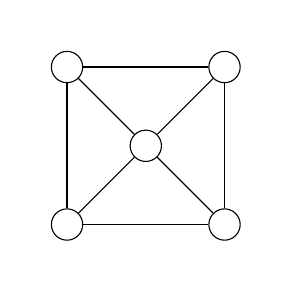
\begin{tikzpicture}[every node/.style={circle, draw, fill=white, inner sep=4pt}]
    \path[use as bounding box] (-0.5,-0.5) rectangle (2.5,2.5);
    \node (A) at (0,0)  {};
    \node (B) at (2,0)  {};
    \node (C) at (2,2)  {};
    \node (D) at (0,2)  {};
    \node (E) at (1,1)  {};

    \draw (A) -- (B) -- (C) -- (D) -- (A);
    \draw (A) -- (E);
    \draw (B) -- (E);
    \draw (C) -- (E);
    \draw (D) -- (E);
    \end{tikzpicture}
    }

    \caption{}
    \label{fig:example-simple}
    \end{subfigure}
    % --- Non-planar graph ---
    \begin{subfigure}{0.25\textwidth}
    \centering
    \resizebox{\linewidth}{!}{
    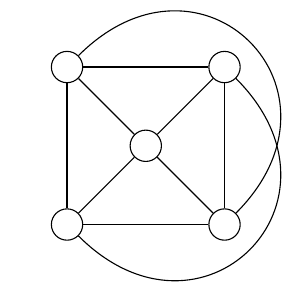
\begin{tikzpicture}[every node/.style={circle, draw, fill=white, inner sep=4pt}]
    \path[use as bounding box] (-0.5,-0.5) rectangle (2.5,2.5);
    \node (A) at (0,0)  {};
    \node (B) at (2,0)  {};
    \node (C) at (2,2)  {};
    \node (D) at (0,2)  {};
    \node (E) at (1,1)  {};

    % Only the cycle highlighted
    \draw (A) -- (B) -- (C) -- (D) -- (A);
    \draw (A) -- (E);
    \draw (B) -- (E);
    \draw (C) -- (E);
    \draw (D) -- (E);
    % Curved outer edges
    \draw[out=-45, in=-45, looseness=2] (A) to (C);
    \draw[out=45, in=45, looseness=2] (B) to (D);

    \end{tikzpicture}
    }

    \caption{}
    \label{fig:example-non-planar}
    \end{subfigure}

    % --- Longest cycle ---
    \begin{subfigure}{0.25\textwidth}
    \centering
    \resizebox{\linewidth}{!}{
    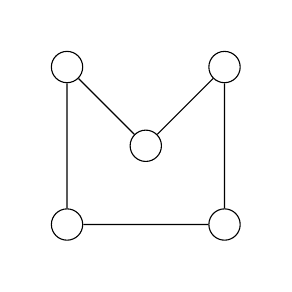
\begin{tikzpicture}[every node/.style={circle, draw, fill=white, inner sep=4pt}]
    \path[use as bounding box] (-0.5,-0.5) rectangle (2.5,2.5);
    \node (A) at (0,0)  {};
    \node (B) at (2,0)  {};
    \node (C) at (2,2)  {};
    \node (D) at (0,2)  {};
    \node (E) at (1,1)  {};

    % Only the cycle highlighted
    \draw (A) -- (B) -- (C) -- (E) -- (D) -- (A);
    \end{tikzpicture}
    }

    \caption{}
    \label{fig:example-cycle}
    \end{subfigure}
    % --- Path ---
    \begin{subfigure}{0.25\textwidth}
    \centering
    \resizebox{\linewidth}{!}{
    \begin{tikzpicture}[every node/.style={circle, draw, fill=white, inner sep=4pt}]
    \path[use as bounding box] (-0.5,-0.5) rectangle (2.5,2.5);
    \node (A) at (0,0)  {};
    \node (C) at (2,2)  {};
    \node (D) at (0,2)  {};
    \node (E) at (1,1)  {};

    % Example path
    \draw (D) -- (A) -- (E) -- (C);
    \end{tikzpicture}
    }

    \caption{}
    \label{fig:example-path}
    \end{subfigure}
    \caption{(\subref*{fig:example-simple}) A simple graph, (\subref*{fig:example-non-planar}) A simple non-planar graph (\subref*{fig:example-cycle}) A cycle, (\subref*{fig:example-path}) A path}
\end{figure}

% Subgraph explanation
A \textbf{subgraph} $F$ of a graph $G$ is a graph for which $V(F) \subset V(G)$ and $E(F) \subset E(G)$, and the edges $E(F)$ only contain vertices in $V(F)$. If the subgraph $F$ is the result of removing one vertex $v$ from $G$ (notation: $G - v$), then we say $F$ is a vertex-deleted subgraph of $G$. Figure \ref{fig:example-cycle} and \ref{fig:example-path} are both subgraphs of \ref{fig:example-simple}\cite{book:bondy-definitions}.

% Cycle explanation
A \textbf{path} is a simple graph whose vertices can be arranged in a linear sequence such that two vertices are adjacent if and only if they are consecutive in the sequence, as shown in figure \ref{fig:example-path}. Similarly, a \textbf{cycle} in a graph is a simple graph whose vertices can be arranged in a linear sequence such that two vertices are adjacent if and only if they are consecutive in the sequence, or they are the first and last vertex in the sequence. The length of a path or cycle is equal to the amount of edges. The \textbf{circumference} of a graph is equal to the length of the longest cycle in the graph. Note that there may be multiple distinct longest cycles. Figure \ref{fig:example-cycle} shows one such longests cycle of the graph in figure \ref{fig:example-simple}\cite{book:bondy-definitions}.

% k-connected
A graph may or may not be connected. A graph is \textbf{connected} if for every partition of vertices into non-empty sets $X, Y$ there exists an edge with one vertex in $X$ and another in $Y$. A graph which is not connected is called disconnected. This concept can be further generalized: a connected graph is \textbf{$k$-vertex-connected} (or simply $k$-connected) if for every pair of distinct vertices $u, v$ it holds that the maximum number of internally disjoint paths from $u$ to $v$ is at least $k$. This should not be confused with the connectivity of a graph, which is the largest value $k$ for which the graph is $k$-connected.
This definition of $k$-connected is equivalent to claiming that a graph is $k$-connected if and only if deleting less than $k$ vertices cannot result in a disconnected graph.
The graph in figure \ref{fig:example-simple} is 3-connected, but not 4-connected, as removing all three vertices on any diagonal would result in a disconnected graph. This graph thus has connectivity 3. Similarly, figure \ref{fig:example-cycle} shows a graph with connectivity 2, and figure \ref{fig:example-path} shows a graph with connectivity 1\cite{book:bondy-definitions}.

\section{Research Questions}
\label{sec:rq}

TODO
